\documentclass[11pt,oneside]{amsart}
\usepackage{geometry}
\geometry{letterpaper}
\usepackage{graphicx}
\usepackage{caption}
\usepackage[singlelinecheck=off,justification=raggedright]{subcaption}
% Change subfigure letters to uppercase
\renewcommand{\thesubfigure}{\Alph{subfigure}}

\usepackage{amssymb}
\usepackage{epstopdf}
\usepackage{natbib}
\usepackage{color}
\usepackage{multirow}
\usepackage{setspace}
\usepackage{xcolor}
\usepackage{tikz}
\usepackage{mathtools}
\usepackage{bbm}


\setlength{\topmargin}{0in}
\setlength{\oddsidemargin}{0in}
\setlength{\textwidth}{6.5in}
\setlength{\textheight}{8.85in}

\RequirePackage{lineno}
\onehalfspacing
\DeclareGraphicsRule{.tif}{png}{.png}{`convert #1 `dirname #1`/`basename #1 .tif`.png}

\bibpunct{(}{)}{,}{a}{}{;}

\newcommand{\E}{\mathbb E}
\newcommand{\Prob}{\mathbb P}
\newcommand{\var}{\text{Var}}
\newcommand{\cov}{\text{Cov}}
\newcommand{\corr}{\text{Corr}}
\newcommand{\nm}{\tilde n_t}
\newcommand{\ns}{\hat n_t}
\newcommand{\nr}{p_t}
\newcommand{\nmtau}{\tilde n_\tau}
\newcommand{\nstau}{\hat n_\tau}
\newcommand{\nrtau}{p_{\tau}}
\newcommand{\Stree}{\mathcal H}
\newcommand{\Gtree}{\mathcal G}
\newcommand{\Top}{\mathcal T}
\newcommand{\Data}{X}
\newcommand{\D}{\mathcal D}
\newcommand{\N}{\mathcal N}
\newcommand{\tcb}{\textcolor{blue}}
\newcommand{\defeq}{\vcentcolon=}

\begin{document}

\linenumbers

\theoremstyle{plain}
\newtheorem{theorem}{Theorem}[section]
\newtheorem{lemma}[theorem]{Lemma}
\newtheorem{corollary}[theorem]{Corollary}
\newtheorem{proposition}[theorem]{Proposition}
\newtheorem{definition}[theorem]{Definition}

\title{Markov Recombination and Migration model}

\maketitle

%\cite{SimonsenChurchill1997}, which extends the coalescent to include recombination, to also include migraiton. Our goal in this project is to build a Markov tree-building model, similar to \cite{SimonsenChurchill1997}, which incorporates both recombination and migration.
%
%Our results include the state space and rates of a continuous time Markov Chain which can be embedded in a discrete time Markov Chain. Here we describe the case of $n = 2$ lineages, which is the case explored by \cite{SimonsenChurchill1997}. We also discuss a combinatorial argument for describing the size of the state space for general $n$.
%
%\Section{Motivation}
%%% Motivation for the problem, Slatkin and Pollack 2008
%
%\cite{SlatkinPollack2008} described how a coalescent model with ancestral population structure could increase the probability of gene-tree species-tree discordance, even potentially making the gene-tree \textit{more} likely than the species tree. 
%

\section{Background}

For a given sample in a model with recombination, the ancestral coalescent tree of a given locus may differ from the ancestral tree of a different locus. For loci that are completely linked, the distribution of trees must be exactly identical. For completely unlinked loci, the distribution of trees for each locus are independent. Previous theoretical work has shown how to construct a set of correlated trees representing the ancestry at linked loci \citep{Hudson1983, Hudson1990, GriffithsMarjoram1996}. \cite{SimonsenChurchill1997} built on the basis of this work by constructing a Markov model for constructing correlated trees with recombination. We expanded on the Markov model developed by \cite{SimonsenChurchill1997} by incorporating population substructure, with two subpopulations with recipricol migration rates, into the model with recombination.

A possible use for this Markov model of recombination and population substructure would be to integrate the results of the model developed by \cite{SlatkinPollack2008}. They showed how ancestral population structure could increase the probability of  gene trees which are discordant with their species trees. They showed that even a simple model with three species, with one sample from each species, some scenarios led to discordant gene trees which were \textit{more} likely than the gene tree concordant with the species tree.

The Markov model constructed in this project which incorporates both recombination and ancestral population structure, could be utilized to analyze how different loci may have ancestral trees that differ in tree height and topology in a model of recombination and population substructure.
%Figure 3 from Slatkin and Pollack 2008

\section{Markov Model with Recombination and Migration}

Like the Simonsen and Churchill, we focused on the case of two sample each sampled at two loci. In the Simonsen and Churchill model, the tree building Markov process transitions between the nine possible states, representing different possible cross sections in time of a genealogy, through a series of coalescent and recombination events. Because there are only 2 samples, there is only one possible topology for the tree.

The different states are determined by a unique tuple $(i, j, k)$ which denotes the number of ``types" that are present at that time. A ``right" type denotes an ancestral sample in which the right locus is ancestral to the one of the original sample and the left locus is not. Similarly a ``left" type denotes when the left locus is ancestral and the right is not. A ``double" is ancestral to one of the present day sample at both loci.

\begin{figure}[ht]
\centering
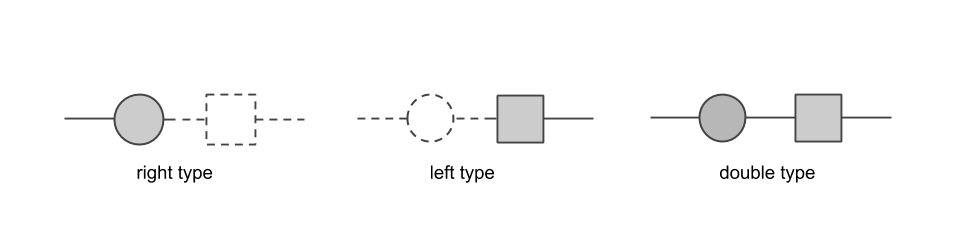
\includegraphics[width=1.0\textwidth]{Terminology.png}
\caption{The states of the Markov chain are determined by the unique tuple denoting the number of right, left, and double types. The colored shapes represent where locus is ancestral to the sample, the empty shapes represent where that locus is not part of the ancestral history being traced.}
\label{Figure: recomb}
\end{figure}

The states can be determined from the possible tuples
\begin{align}
1 &\leq i+k \leq 2 \label{Eqn: i + k leq 2} \\
1 &\leq j+k \leq 2 \label{Eqn: j + k leq 2}  \\
0 &\leq i,j,k \label{Eqn: all geq 0}
\end{align}

Eq. (\ref{Eqn: i + k leq 2}) are true because each left locus ancestral to a sample must either be contained in a left type or a double and there is are two sampled left loci until they coalesce into 1. The same reasoning determines eq. (\ref{Eqn: j + k leq 2}) for the right locus. Given these constraints, there are 9 states.

As in the standard coalescent model, in the Simonsen and Churchill model, the assumption that probability of multiple events occurring simultaneously can be ignored. 

The transitions are defined by either recombination-- in which a double becomes a right and left type at the next state-- or coalescent events-- where two lineages reduce to one (a right and left type become one double, a right or left and a double become a double, and two of any one type reduce to one lineage after a coalescent event). The rate of coalescence, scaled by the population size is 1. The rate of recombination, scaled by the population size is R. In the discrete case, the time until transition is ignored and transition probabilities are determined proportional to the rate of transition to each state in the continuous case.

\begin{figure}[ht]
\centering
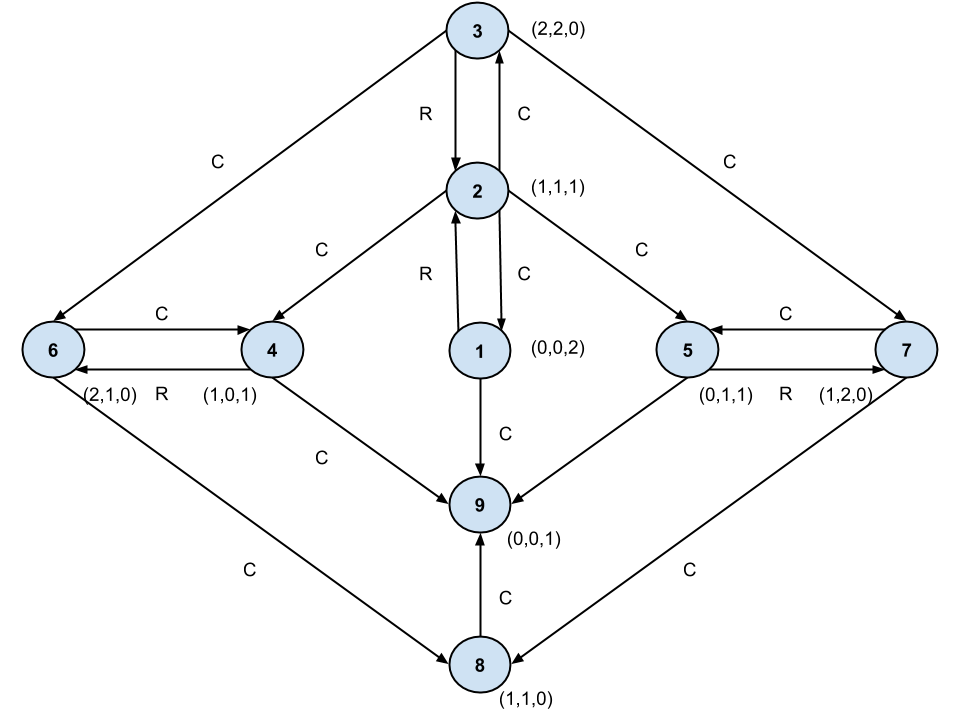
\includegraphics[width=0.75\textwidth]{Markov_recomb.png}
\caption{Full state space for model with just recombination (Figure 3 from \cite{SimonsenChurchill1997}).}
\label{Figure: recomb}
\end{figure}
	
\subsection{Extending model to recombination and migration, $n = 2$.}

To extend this model to include population substructure, the states in the model incorporate information about which population each lineage in the cross section resides at that cross section in time. From the nine states in the original Simonsen and Churchill model with two samples and two loci, the extended population substructure and recombination Markov chain includes 46 states. The process can transition between state by coalescence, recombination, and migration. Two lineages can only coalesce at a given if they are currently in the same population.
\begin{figure}[ht]
\centering
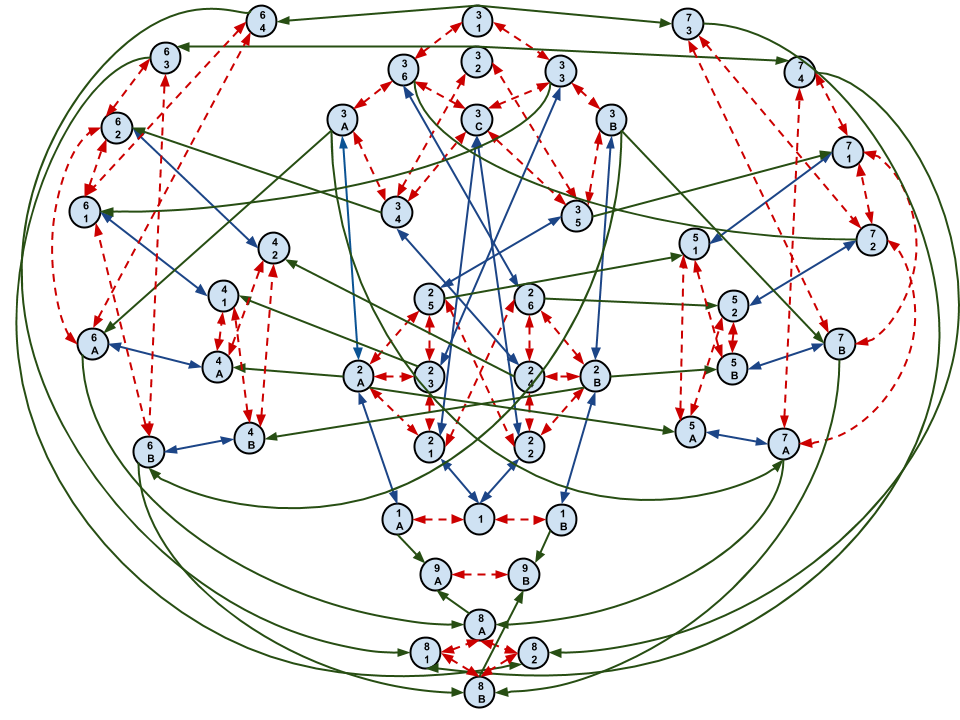
\includegraphics[width=1.0\textwidth]{Markov_recomb_mig.png}
\caption{Full state space for model with recombination and migration.}
\label{Figure: recomb mig}
\end{figure}

\subsection{Probability of equal tree height.}

The matrix defined by the Markov chain for the model with population substructure and recombination can be used to simulate the Markov chain of the model with population substructure and recombination. We compared the probability of equal tree height as it changes with recombination rate for the Simonsen and Churchill model and the extended model with population structure. Simonsen and Churchill also show a scatter plot of simulated left and right tree heights given a population recombination rate, R = 2N*r = 0.723, the value for which the probabilities of equal and unequal tree heights are approximately equal to the probabilty of unequal tree heights. If the tree heights are unequal, either loci is equally likely to be the taller one. We have done the same simulation for the extended model.

Simulations for the extended model show how the probability of equal tree heights changes with recombination rate R = 20, 10, 5, 2, 1, 0.1, 0.01, 0.001. The analytical solution to the probability of equal tree height was found analytically by \cite{Griffiths1981} and utilized in the Simonsen and Churchill paper. Points represent the output of equal tree height measured from simulation and the lines show how the probability of equal tree heights changes in the original model with increasing R, found analytically.  
%In the Simonsen and Churchill model, the analysis requires finding the probability of the confining the process to three states before it reaches the absorbing state. The analogous analysis in the extended model requires accounting for the probability of remaining in nineteen states and therefore can be solved for by solving a system of nineteen equations. Both figures show how from intermediate values of R, the extended model with population structure has a lower probability of equal tree heights at both loci.

\begin{figure}[ht]
\centering
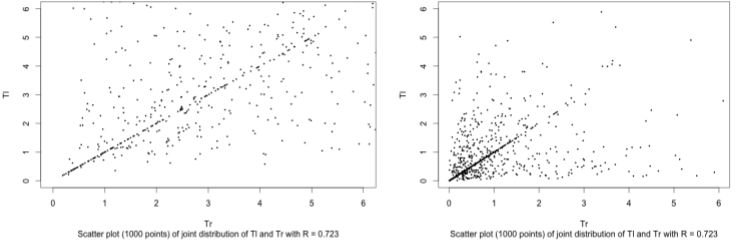
\includegraphics[width=1.0\textwidth]{Dst_height.png}
\caption{Distribution of different tree heights, generated from simulated runs of the Markov model for the recombination-only and the recombination and migration model.}
\label{Figure: n = 3 lumped recomb}
\end{figure}

\begin{figure}[ht]
\centering
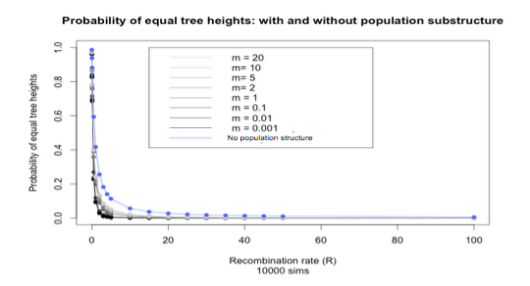
\includegraphics[width=0.75\textwidth]{Pequal_height.png}
\caption{Probability of equal tree heights for different mgirations rates, $m$.}
\label{pequal height}
\end{figure}


\subsection{Number of states for $n$ samples.}

Ignoring topology, extending the Simonsen and Churchill model to include $n$ samples and 2 loci,  we used a combinatorial argument to find the number of states in the model given a value of n by considering the types of lineages possible and and considering different configurations based on the position of these lineages in different populations. Based on this combinatorial reasoning, we obtained an expression with three sums, for S(n), the number of states in the model given n:
\begin{equation}
S(n) = \sum^{n}_{z = 0} \Bigg( (n-z+1)\bigg[\Big(\sum^{z}_{y = 1} (y+1)\Big)^2 + \mathbbm{1}\{n-z > 0\}(1+2\bigg(\sum^z_{y = 1}(y+1)\Big) \bigg] \Bigg)
\label{Eqn: combinatorial count}
\end{equation}

We used Faulhaber’s formulas to simplify the expression to find the closed form expression is below.
\begin{equation}
S(n) = n^6/120+n^5/8+(3*n^4)/4+(55*n^3)/24+(329*n^2)/120+n/12
\label{Eqn: combinatorial count Fauhaber formula}
\end{equation}

Though not growing exponentially, this formula shows that incorporating more samples into the model, even ignoring topology, may be challenging. The minimal interesting case to combine the model with \cite{SlatkinPollack2008} would be $n = 3$, meaning the extended \cite{SimonsenChurchill1997} model with population substructure would have 184 states. %It may however be possible write a program to generate these states and the corresponding transition matrix using combinatorics. Further analysis would be needed however to consider how best to include topology in order to answer this question. 

\subsection{The lumped model and $n = 3$.}

Partitioning a Markov chain into subsets of states, also referred to as ``lumping" a Markov chain, reduces the number of states. A continuous-time Markov chain is lumpable with respect to a partition if and only if, for any subsets $T_i$ and $T_j$ in the partition, and for any states $n$, $n'$ in subset $T_i$, where $P(i,j)$ is the transition probability from state $i$ to state $j$,
\begin{equation}
\sum_{m \in T_j} P(n, m) = \sum_{m \in T_j} P(n', m)
\label{Eqn: lumpability}
\end{equation}

Similarly, the same condition holds for rates instead of probabilities when the Markov chain is continunous time.

Lumpability is useful in this project to reduce the size of state-space due to the different symmetries which can be ignored: the transitions and states are respectively the same for each loci (right or left) and each population (A or B) and transitions to symmetric states are mutually exclusive.

The lumped space from the \cite{SimonsenChurchill1997} model can be used to elucidate the state space of $n=3$, without population structure. State-space represented in its ``lumped" space can be deconstructed into the unlumped space. 

It may be possible to ``un-lump" the $n=3$ model to include topology, which could be interesting for combining with the \cite{SlatkinPollack2008}

%% Lumping -- easier to add migration, add add topology for n =3
%% n = 3 (lumpy space)

% Hudson, R. R. 1983. Properties of a neutral allele model with intragenic recombination, Theoretical Population Biology 23, 183-201.

% Hudson, R. R. 1990. Gene genealogies and the coalescent process, Oxford Suverys in Evolutionary Biology 7, 1-44.

% Dutheil, Julien Y., et al. Ancestral Population Genomics: The Coalescent Hidden Markov Model Approach. Genetics 183 (2009): 259-74. 

% Griffiths, R. C. 1981. Neutral two-locus multiple allele models with recombination, Theoretical Population Biology 19, 169-186.

\begin{figure}[ht]
\centering
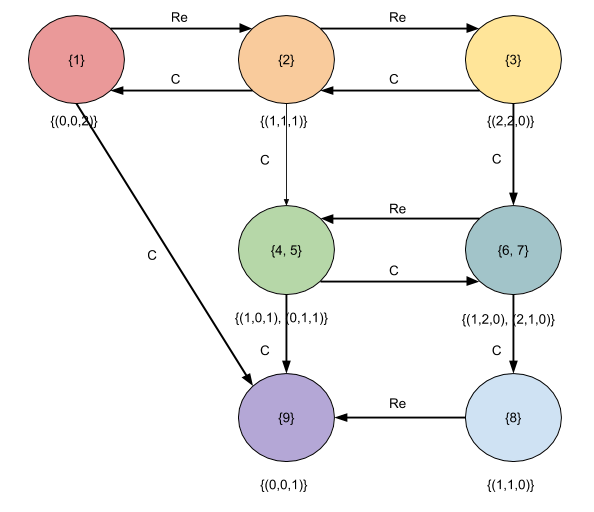
\includegraphics[width=0.5\textwidth]{Lumped_recomb.png}
\caption{Lumped Markov chain in model with recombination, no substructure.}
\label{Figure: lumped recomb}
\end{figure}

\begin{figure}[ht]
\centering
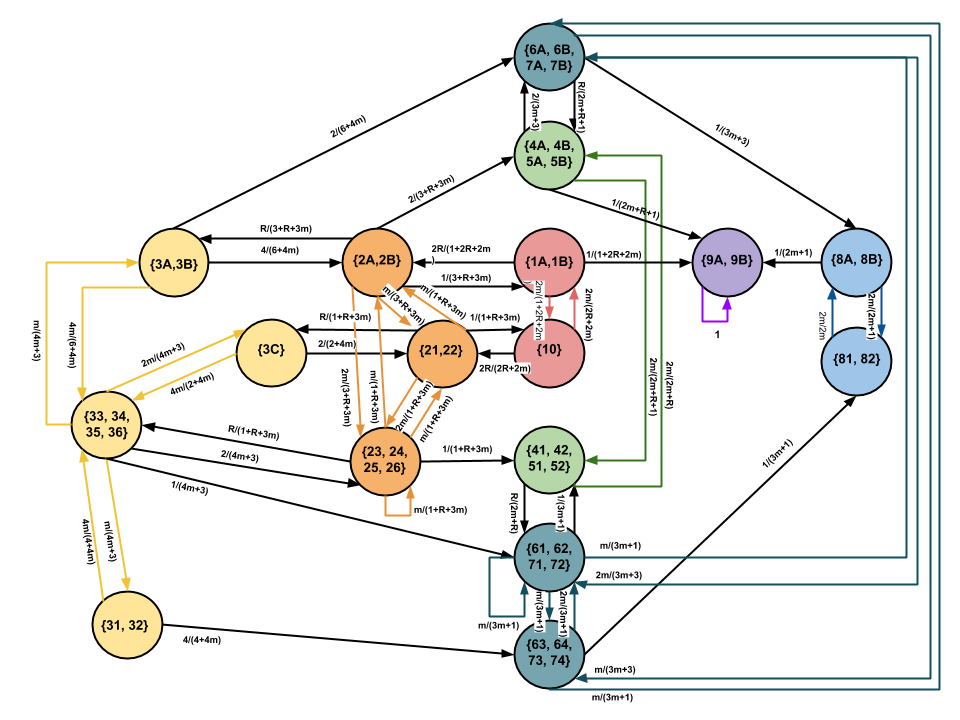
\includegraphics[width=1.00\textwidth]{Lumped_RecombMig.png}
\caption{Lumped Markov chain in model with recombination and substructure.}
\label{Figure: lumped recomb mig}
\end{figure}

\begin{figure}[ht]
\centering
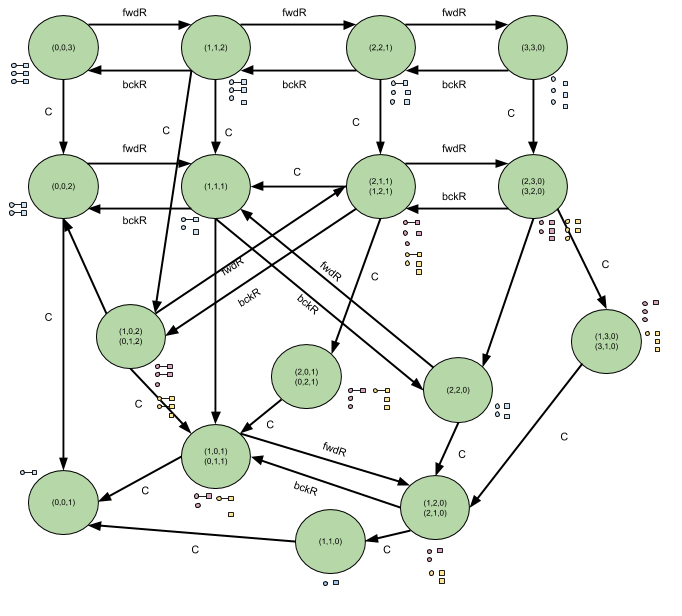
\includegraphics[width=1.0\textwidth]{n3_notopology_lumped_recomb.png}
\caption{Lumped state space for $n = 3$ with recombination, no substructure.}
\label{Figure: n = 3 lumped recomb}
\end{figure}

\clearpage

\vskip .4cm
\begin{small}
\bibliographystyle{chicago}
\bibliography{Markov_ReMig.bib}
%\bibliographystyle{plainnat}
%\bibliography{Intro}
\end{small}


\end{document}